\documentclass[a4paper,12pt]{article}

\usepackage[T1]{fontenc}
\usepackage[utf8]{inputenc}
\usepackage[english, polish]{babel}
\usepackage{lmodern}
\usepackage{graphicx}
\usepackage{fancyhdr}
\usepackage{float}
\usepackage{array}
\usepackage{hyperref}
%\usepackage{mathtools}


\setlength{\textheight}{23.5cm}
\setlength{\textwidth}{15.92cm}
\setlength{\footskip}{10mm}
\setlength{\oddsidemargin}{0mm}
\setlength{\evensidemargin}{0mm}
\setlength{\topmargin}{0mm}
\setlength{\headsep}{15mm}
\setlength{\parindent}{0cm}
\setlength{\parskip}{2.5mm}
%nowa extra row do tabeli :)  :) 
\setlength{\extrarowheight}{4pt}

\author{Justyna Ilczuk, Jacek Rosiński}

\begin{document}

\begin{center}

    \begin{tabular}{ | m{5cm}| m{5cm} | m{5cm} |}
    \hline 
    \multicolumn{2}{|c|}{{ \Large \textbf{Laboratorium Fizyki 2}} }
    &  
    \begin{center}
    Data wykonania ćwiczenia:
    \end{center}
    \begin{center}
      16.10.2013 
    \end{center}
    \begin{center}
    Środa 9.45-12.45
    \end{center}
     \\ 
    
    \hline
    \multicolumn{2}{|c|}{Justyna Ilczuk \newline Jacek Rosiński}
    & \begin{center}
    {\small Data złożenia sprawozdania:} \newline \today
    \end{center}   \\
   	
   	\hline
    Wydział Fizyki & Grupa: K-1 \newline Rok akademicki: 2013/2014 &  \\
   	\hline
   	\multicolumn{2}{|l|}{Prowadzący: Michał Marzanotowicz} & \multicolumn{1}{|l|}{Ocena końcowa:}\\
    \hline
    \end{tabular}
\end{center}

\newpage

\pagestyle{fancy}
\fancyfoot[CO]{\ }
\fancyhead[RO]{\footnotesize{\thepage} }
%\fancyhead[RO]{\footnotesize{\ } }
\fancyhead[LO]{Justyna Ilczuk i Jacek Rosiński K-1, Ogniwo DMFC }

% wrzucanie wykresów:

%\begin{figure} [H]
%  \begin{center}
%    \includegraphics[width = 15cm]{Rysunek.png}
%    \caption{Układ pomiarowy}
%  \end{center}
%\end{figure}


\section{Cel ćwiczenia}

Celem naszego ćwiczenia projektowego było naprawienie ogniwa metanolowego. Ogniwo, które otrzymaliśmy miało bardzo niską sprawność i można było z niego pobierać moc rzędu wielkości mikro watów.



\section{Wstęp}

Ogniwo z jakim mieliśmy do czynienia nazywa się Direct Methanol Fuel Cell - paliwem w nim jest 3$\%$ roztwór metanolu.

Podstawowym wyznacznikiem naprawienia ogniwa, było to, żeby mogło zasilać dołączony do niego wiatraczek.

Ważnymi parametrami ogniwa są:
\begin{itemize}
\item oporność wewnętrzna
\item moc
\item napięcie maksymalne
\end{itemize}
\section{Użyty sprzęt i układy pomiarowe}

W naszym ćwiczeniu używaliśmy:
\begin{itemize}
\item komputera i automatycznego miernika napięcia
\item metanolu i kwasu siarkowego VI
\item mierników uniwersalnych
\item oporników dekadowych
\item wagi precyzyjnej (która podczas trwania badań przestała jednak działać)
\end{itemize}

\section{Przebieg ćwiczenia i opracowanie wyników}

%Na początku zmierzyliśmy charakterystyki ogniwa dla róznych zawartości metanolu w paliwie:


%Tu wrzucimy wykresy z pierwszego sheet'a w gnumericu expotent

By zwiększyć wydajność ogniwa wykonaliśmy na nim różne zabiegi:
\begin{itemize}
\item zwilżanie membrany (nafionowej)
\item przemywanie membrany pod strumieniem wody
\item ogrzewanie
\item kolejne cykle z nowym paliwem
\item "kąpiel" w rozcięczonym kwasie siarkowym VI
\end{itemize}

Zwilżanie membrany polepsza parametry ogniwa. Musi być jednak wykonane w odpowiedni sposób. Najlepszym ze sprawdzonych przez nas sposobów było zmoczenie bezpośrednie membrany poprzez naniesienie kilku kropel wody i odczekanie kilku chwil.

Największy wpływ na parametry ogniwa miały kolejne cykle pracy. Każde kolejne badanie charakterystyk pokazywało, że wydajność wzrasta, a poór wewnętrzny spada. Sugeruje to, że membrana nafionowa poprzez pozostawanie przez długi okres czasu nienawilżana, po woli traciła zdolność do przepuszczania jonów $H^+$. Jako że Nafion jest materiałem polarnym, mógł się 'zapchać' drobinkami kurzu, który blokował dopływ metanolu.

Bardzo dobry skutek na ogniwo wywarła "kąpiel" w rozcięczonym ($1\%$) kwasie siarkowym (VI) ($ H_2SO_4 $).

Przed przeprowadzeniem szeregu zabiegów moc uzyskiwana przez ogniwo w zależności od natężenia prądu przedstawiała się następująco

\begin{figure} [H]
 \begin{center}
    \includegraphics[width = 15cm]{przed.png}
   % \caption{Charakterystyka dla 3$\%$ roztworu metanolu i }
  \end{center}
\end{figure}
Niepokojący był fakt, że moc uzyskana dla roztworu o słabszym stężeniu paliwa miał większą wydajność. Jak się okazało, to ogniwo, dzięki kolejnym cyklom pracy, funkcjonowało coraz lepiej. Jednak nie było zdolne do zasilenia wiatraczka. Opór wewnętrzny okniwa wynosił $80 \Omega $


Próbowaliśmy na kilka sposobów polepszyć nasze statystyki. Najlepszym sposobem na to okazało się całonocne moczenie membrany z roztworek bardzo katywnego chemicznie $ H_2SO_4 $. 

Charakterystyki wówczas lekko się zmieniły. Opór wewnętrzny zmalał do $30 \Omega $ zaś wykres mocy w zależności od natężenia znacząco zmieniły. Wartości mocy wzrosły czterokrotnie. 
\begin{figure} [H]
 \begin{center}
    \includegraphics[width = 15cm]{po.png}
   % \caption{Charakterystyka dla 3$\%$ roztworu metanolu i }
  \end{center}
\end{figure}

Interesowały nas także charakterystyki zużycia paliwa i napięcia od czasu.

Zmierzyliśmy takie charakterystyki dla trzech wartości zawartości paliwa: $3\%$, $2\%$, i $1\%$ na oporze $30 \Omega $, ponieważ to był opór, dla jakiego ogniwo uzyskiwało największą moc. 

\begin{figure} [H]
 \begin{center}
    \includegraphics[width = 15cm]{DMFC_U(T).png}
    %\caption{Układ pomiarowy}
  \end{center}
\end{figure}

Widzimy, że dla paliwa z $3\%$ roztworem metanolu napięcie utrzymywane przez ogniwo było stałe przez 4 godziny. Następnie zaczęło spadać. Dla $2\%$ roztworu metanolu proces obniżania się napięcia występował od razu po podłączeniu do układu pomiarowego, stąd wniosek, że przy pomiarze charakterystyki $3\%$ stałe napięcie utrzymuje się dopóki stężenie metanolu jest większe niż $2\%$. Po przekroczeniu tej wartości metanol nie nadąża dyfundować do membrany, w ilości zapewniającej działanie ogniwa na pełnej mocy, zaś paliwo dalej się zużywa, aż do całkowitego wykończenia. Pomiar $1\%$ roztworu miał wiele zakłóceń, i jego wykres znacząco odbiga od innych. Może być to związane z większą ilością wody w próbce, przez co metanol miał trudniejszą drogę do pokonania. Zmniejszyło to nachylenie krzywej na wykresie. Końcówka wykresu jest całkiem inna od pozostałych. Ponieważ pomiar trwał  kilka godzin, poderzewamy, że ktoś przewrócił ogniwo i wyciekło z niego paliwo.

Niestety, waga jakiej używaliśmy do sporządzania roztworów przestała działać w trakcie laboratoriów i nie mogliśmy zważyć ile paliwa używaliśmy w doświadczeniu. 

Najważniejsze parametry ogniwa:
\begin{itemize}
  \item $ P_{max}= 2.8 mW $
  \item $U_{max}= 0.6 V $
  \item $I_{max}= 24.8 mA$
  \item $r_{w}= 30 \Omega$
  \item $t_{rozł}= 4 h $
\end{itemize}
Gdyby do ogniwa wchodziło 2ml paliwa, wówczas samego metanolu było by 0.06 g. Przrzez piersze 4 godziny działania przez układ płynie stały prąd 8.1 mA. Można stąd wyliczyć pojemność grawimetryczną ogniwa z paliwem, jak dla baterii:
$$ Q = \frac{q}{m} =\frac{It}{m}= \frac{8.1 \cdot 4}{0.06}= 540 \frac{mAh}{g} $$



\section{Wnioski}
Udało nam się doprowadzić ogniwo do stanu w którym może napędzać wiatraczek. Dobrym roztworem czyszczącym jest rozcieńczony kwas siarkowy. Membrana nafionowa powinna być przechowywana przy zachowaniu dużej wilgotności, zaś ogniwo powinno być od czasu do czasu używane, aby 'rozruszać' membranę. Nafion lepiej działa gdy jest wcześniej odpowiednio zwilżony. Ogniwa DMFC mają potencjalnie spory szereg zastosowań, jednak ciężka dostępność metanolu i wysoki koszt membrany, nie ułatwiją korzystania z tego rodzaju źródeł prądu. 

\end{document}
